\documentclass[
11pt, % The default document font size, options: 10pt, 11pt, 12pt
%codirector, % Uncomment to add a codirector to the title page
]{charter} 


% El títulos de la memoria, se usa en la carátula y se puede usar el cualquier lugar del documento con el comando \ttitle
\titulo{Monitoreo y predicción in-situ de propiedades mecánicas en fabricación aditiva de fibra continua con materiales compuestos} 

% Nombre del posgrado, se usa en la carátula y se puede usar el cualquier lugar del documento con el comando \degreename
%\posgrado{Carrera de Especialización en Sistemas Embebidos} 
%\posgrado{Carrera de Especialización en Internet de las Cosas} 
%\posgrado{Carrera de Especialización en Inteligencia Artificial}
%\posgrado{Maestría en Sistemas Embebidos} 
%\posgrado{Maestría en Internet de las cosas}
\posgrado{Maestría en Computación de Borde}

% Tu nombre, se puede usar el cualquier lugar del documento con el comando \authorname
% IMPORTANTE: no omitir titulaciones ni tildación en los nombres, también se recomienda escribir los nombres completos (tal cual los tienen en su documento)
\autor{Ing. Simón A. Rodríguez Alzuru}

% El nombre del director y co-director, se puede usar el cualquier lugar del documento con el comando \supname y \cosupname y \pertesupname y \pertecosupname
\director{\textcolor{red}{Título y Nombre del director}}
\pertenenciaDirector{\textcolor{red}{pertenencia}} 
\codirector{} % para que aparezca en la portada se debe descomentar la opción codirector en los parámetros de documentclass
\pertenenciaCoDirector{FIUBA}

% Nombre del cliente, quien va a aprobar los resultados del proyecto, se puede usar con el comando \clientename y \empclientename
\cliente{M.Sc. Jan Seiffert}
\empresaCliente{Decanato Materiales Compuestos (TUM)}
 
\fechaINICIO{24 de junio de 2025}		%Fecha de inicio de la cursada de GdP \fechaInicioName
\fechaFINALPlan{20 de agosto de 2025} 	%Fecha de final de cursada de GdP
\fechaFINALTrabajo{\textcolor{red}{xx de mayo} de 2026}	%Fecha de defensa pública del trabajo final


\begin{document}

\maketitle
\thispagestyle{empty}
\pagebreak


\thispagestyle{empty}
{\setlength{\parskip}{0pt}
\tableofcontents{}
}
\pagebreak


\section*{Registros de cambios}
\label{sec:registro}


\begin{table}[ht]
\label{tab:registro}
\centering
\begin{tabularx}{\linewidth}{@{}|c|X|c|@{}}
\hline
\rowcolor[HTML]{C0C0C0} 
Revisión & \multicolumn{1}{c|}{\cellcolor[HTML]{C0C0C0}Detalles de los cambios realizados} & Fecha      \\ \hline
0      & Creación del documento                                 &\fechaInicioName \\ \hline
1      & Se completa hasta el punto 5 inclusive                & {08} de {julio} de 2025 \\ \hline
2      & Se completa hasta el punto 9 inclusive                & {15} de {julio} de 2026 \\ \hline
%3      & Se completa hasta el punto 12 inclusive                & {día} de {mes} de 202X \\ \hline
%4      & Se completa el plan	                                 
%		  Se puede agregar algo más \newline
%		  En distintas líneas \newline
%		  Así                                                    & {día} de {mes} de 202X \\ \hline


% Si hay más correcciones pasada la versión 4 también se deben especificar acá

\end{tabularx}
\end{table}

\pagebreak



\section*{Acta de constitución del proyecto}
\label{sec:acta}

\begin{flushright}
Buenos Aires, \fechaInicioName
\end{flushright}

\vspace{2cm}

Por medio de la presente se acuerda con el \authorname\hspace{1px} que su Trabajo Final de la \degreename\hspace{1px} se titulará ``\ttitle'' y consistirá en el monitoreo en tiempo real de las condiciones de impresión y la predicción in situ de las propiedades mecánicas de las partes fabricadas durante el proceso de impresión. El trabajo tendrá un presupuesto preliminar estimado de 663 horas, con fecha de inicio el \fechaInicioName\hspace{1px} y fecha de presentación pública el \fechaFinalName.

Se adjunta a esta acta la planificación inicial.

\vfill

% Esta parte se construye sola con la información que hayan cargado en el preámbulo del documento y no debe modificarla
\begin{table}[ht]
\centering
\begin{tabular}{ccc}
\begin{tabular}[c]{@{}c@{}}Dr. Ing. Ariel Lutenberg \\ Director posgrado FIUBA\end{tabular} & \hspace{2cm} & \begin{tabular}[c]{@{}c@{}}\clientename \\ \empclientename \end{tabular} \vspace{2.5cm} \\ 
\multicolumn{3}{c}{\begin{tabular}[c]{@{}c@{}} \supname \\ Director del Trabajo Final\end{tabular}} \vspace{2.5cm} \\
\end{tabular}
\end{table}




\section{1. Descripción técnica-conceptual del proyecto a realizar}
\label{sec:descripcion}

El proyecto se realiza para el Decanato de materiales compuestos de la escuela de ingeniería y diseño de la Universidad Técnica de Múnich en Alemania, el cual investiga el desarrollo de nuevos métodos y conceptos para la fabricación aditiva continua reforzada por fibra. Uno de los métodos investigados es el proceso de fabricación con filamento fundido (FFF), también conocido como modelado por deposición fundida. Este proceso es ideal para producir prototipos funcionales ligeros y permite, por ejemplo, la integración de sensores o de refuerzos orientados a una carga al utilizar fibras reforzantes. 

Integrar adecuadamente estas fibras y sensores es esencial para la producción de componentes estructurales. Por lo tanto, es crucial tener un proceso de monitoreo automatizado durante la producción de dichos componentes para validar su calidad y generar un gemelo digital que pueda ser utilizado para predecir las propiedades mecánicas de las partes impresas.

Actualmente se utilizan métodos de elementos finitos para el análisis y predicción de propiedades mecánicas de las partes impresas; una actividad que requiere gran poder de cómputo, consume mucho tiempo y, por lo tanto, no se realiza en tiempo real. Este proyecto busca una alternativa para predecir las propiedades mecánicas de las partes impresas desde el primer instante del proceso de impresión. Se implementa, además, una interfaz para la visualización y monitoreo continuos del proceso, que incluye las desviaciones de la fibra y los resultados de predicción de sus propiedades.

En la figura \ref{fig:procesoActual} se muestra el estado actual del sistema y el proceso que se desarrolló en un trabajo previo dentro del decanato y sobre el cual se basa el presente proyecto. Se puede observar que se cuenta con una impresora 3D multiherramienta con capacidad de visión por computadora a través de una cámara y una Raspberry Pi. La herramienta de visión captura imágenes automáticamente de la deposición de la fibra, de donde puede obtenerse información sobre la posición de la fibra y sus defectos. Una computadora conectada a la impresora y a la herramienta de visión controla el proceso de captura de imágenes y las almacena localmente.

\begin{figure}[htpb]
\centering 
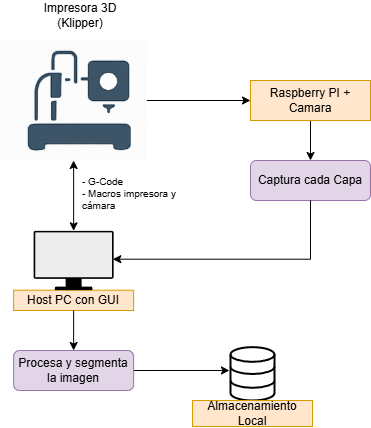
\includegraphics[width=.5\textwidth]{Figuras/proceso-Actual.png}
\caption{Diagrama del proceso actual.}
\label{fig:procesoActual}
\end{figure}

El sistema almacena las imágenes capturadas para su análisis posterior y no posee capacidades para realizar un análisis en tiempo real de éstas ni analiza las propiedades mecánicas de las partes impresas. El sistema tampoco incluye el monitoreo en tiempo real del proceso de impresión y el acceso al panel de control se realiza únicamente de forma local. Por último, no existen automatizaciones para el proceso de impresión.

Para mejorar el proceso y solucionar estas brechas, se propone analizar dos métodos de inteligencia artificial diferentes para predecir propiedades mecánicas (p.ej. rigidez, resistencia, coeficiente de Poisson) en base a imágenes. Estos modelos deben entrenarse con las imágenes disponibles, parámetros de impresión, resultados experimentales y datos de simulación. Posteriormente, los resultados se evalúan con datos de prueba nuevos y se comparan con resultados experimentales y predicciones por simulación, para finalmente elegir el mejor método a implementar.

Adicionalmente, para mejorar las capacidades de control y monitoreo del proceso de impresión se propone implementar la visualización en tiempo real del proceso en un \textit{dashboard} que incluya la predicción de las propiedades mecánicas por IA. Por último, para facilitar el acceso al panel, se propone agregar al sistema el envío de telemetría durante el proceso de impresión.

En la figura \ref{fig:procesoPropuesta} se observa el nuevo proceso propuesto que incluye la predicción de las propiedades mecánicas, el monitoreo en tiempo real del proceso de impresión y la transmisión de telemetría para su consumo remoto. 

\begin{figure}[htpb]
\centering 
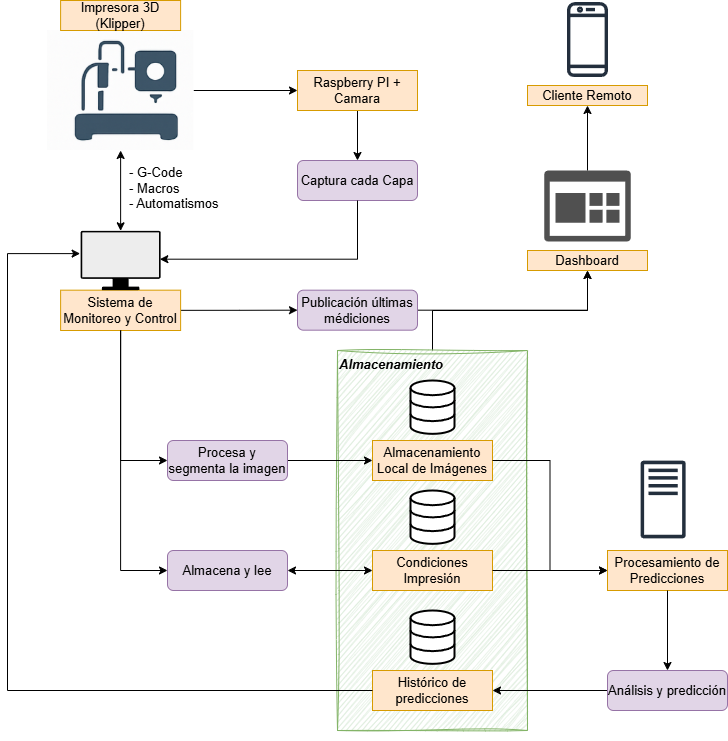
\includegraphics[width=.8\textwidth]{Figuras/proceso-Propuesto.png}
\caption{Propuesta del proyecto.}
\label{fig:procesoPropuesta}
\end{figure}

Se propone segmentar los datos en distintos medios de almacenamiento (imágenes, propiedades de impresión, predicciones, etc.) para facilitar su administración y acceso. Se puede observar además que el \textit{dashboard} para acceso remoto consumirá datos tanto de las bases de datos (por ejemplo, históricos), como también directamente del sistema de monitoreo y control a través de la transmisión de los últimos datos de telemetría.

Este trabajo se realiza en las instalaciones de la Universidad Técnica de Múnich en el área de laboratorio dispuesta por el decanato para la impresión de partes por el método de fabricación con filamento fundido, así como dentro de la red científica interna de Múnich (MWN, o \textit{Münchener Wissenschafts Netz)}.


\section{2. Identificación y análisis de los interesados}
\label{sec:interesados}

\begin{table}[ht]
%\caption{Identificación de los interesados}
%\label{tab:interesados}
\begin{tabularx}{\linewidth}{@{}|l|X|X|l|@{}}
\hline
\rowcolor[HTML]{C0C0C0} 
Rol           & Nombre y Apellido & Organización 	& Puesto 	\\ \hline
Cliente       & \clientename      &\empclientename	& Líder IA y Digitalización      	\\ \hline
Responsable   & \authorname       & FIUBA        	& Alumno 	\\ \hline
Orientador    & \supname	      & \pertesupname 	& Director del Trabajo Final \\ \hline
Usuario final & Estudiantes y Personal                  & TUM             	&  -      	\\ \hline
\end{tabularx}
\end{table}

\begin{itemize}
	\item Orientador: \textcolor{red}{pendiente a definir.}
	\item Cliente: \clientename{} es el líder del tema inteligencia artificial y digitalización del decanato de materiales compuestos en la TUM e investigador/doctorando. Se encarga de liderar y desarrollar investigaciones en esta área. Conoce muy bien los temas de materiales compuestos y mecánica aeroespacial, pero su conocimiento en IoT no es profundo. Apoya el proyecto con conocimiento técnico y soporte a la investigación, además de acceso a los recursos de la universidad.
	\item Usuario final: si bien los usuarios finales actuales son estudiantes y personal que hace vida en el decanato de materiales compuestos, se puede expandir a usuarios finales dentro de la industria.
\end{itemize}


\section{3. Propósito del proyecto}
\label{sec:proposito}

El objetivo de este trabajo es utilizar métodos de inteligencia artificial para predecir in-situ, y durante el proceso de impresión, propiedades mecánicas de partes impresas por fabricación aditiva reforzada con fibra. Así como el monitoreo en tiempo real de forma local y a distancia del proceso de impresión. 


\section{4. Alcance del proyecto}
\label{sec:alcance}

El proyecto incluye:
\begin{itemize}
	\item Análisis de los datos disponibles, procesos y códigos.
	\item Selección de un método de inteligencia artificial para predecir las propiedades mecánicas de partes hechas por fabricación aditiva reforzada con fibra.
		\begin{itemize}
		\item Preselección de métodos diferentes para la predicción de las propiedades mecánicas.
        \item Preparación de los \textit{datasets} para el entrenamiento de los modelos con apoyo del cliente.
		\item Entrenamiento de los modelos preseleccionados con datos disponibles: imágenes segmentadas, parámetros de impresión, resultados experimentales, datos de simulación.
		\item Evaluación de los modelos de inteligencia artificial con resultados de pruebas experimentales y predicciones por simulación.
        \item Selección del mejor método de inteligencia artificial.
		\end{itemize}
    \item Predicción de propiedades mecánicas durante el proceso de impresión en base a imágenes capturadas y datos de impresión.
	\item Mejora de la interfaz de usuario existente para mostrar los datos de la predicción en tiempo real.
    \item Transmisión en tiempo real de datos de telemetría del proceso de impresión.
    \item Acceso remoto a datos de telemetría en tiempo real y datos históricos.
    \item Reestructuración de la arquitectura del sistema para almacenar datos históricos y permitir procesos de automatización y monitoreo avanzados.
    \item Reestructuración del proceso y flujo de datos.
    \item Propuesta de automatización en base a datos del proceso de impresión.
	
\end{itemize}

El presente proyecto no incluye la preparación y configuración del equipo de impresión ni de la herramienta de captura de imágenes. En caso de ser necesaria la captura de más datos o imágenes, el cliente se encargará de obtener todos los datos necesarios para el entrenamiento y validación de los modelos, incluyendo resultados de pruebas o simulaciones. 

Por último, pueden existir modificaciones al alcance del proyecto debido a nuevos descubrimientos durante la ejecución del trabajo, en cuyo caso, serán analizadas individualmente, estimado su impacto, y se tomará una decisión al respecto con el acuerdo de todas las partes interesadas.


\section{5. Supuestos del proyecto}
\label{sec:supuestos}

Para el desarrollo del proyecto se supone lo siguiente:

\begin{itemize}
	\item Se dispone del acceso a las instalaciones donde se encuentra el sistema (impresora, herramienta de visión, PC, código, etc.).
	\item Se cuenta con acceso a todos los datos necesarios para el entrenamiento y evaluación de los modelos de inteligencia artificial, y en caso de faltar o requerir más datos, el cliente dispondrá de los mismos.
	\item Se tiene acceso a equipos para el entrenamiento y validación de los modelos. El equipo para la inferencia/predicción de las propiedades mecánicas también se encuentra disponible o puede conseguirse antes de finalizar el proyecto.
    \item El cliente dará apoyo y supervisión in-situ durante el proyecto.
    \item El proyecto se realiza a tiempo parcial de forma híbrida (combinación in-situ y remoto).
\end{itemize}

\section{6. Requerimientos}
\label{sec:requerimientos}

\begin{enumerate}
	\item Requerimientos funcionales:
		\begin{enumerate}
			\item El sistema debe poder predecir las propiedades mecánicas de una parte impresa durante el proceso de impresión.
			\item El sistema debe poder procesar la información de cada una de las capas de impresión (imágenes, segmentación, propiedades y condiciones de impresión) para realizar la predicción de las propiedades mecánicas de la pieza.
			\item El usuario no debe realizar ninguna operación especial para obtener los resultados de las predicciones de la pieza que se está imprimiendo.
            \item El sistema debe almacenar los resultados históricos de predicción para que el usuario pueda visualizarlos cuando lo desee.
            \item El sistema debe integrarse a la interfaz local existente y al proceso del sistema actual sin realizar cambios fundamentales al proceso de impresión (de ser posible).
            \item El usuario debe poder acceder remotamente a los resultados en directo, vía alguna interfaz simplificada.
            \item El usuario debe poder acceder remotamente a los resultados históricos.
		\end{enumerate}
    \item Requerimientos de la interfaz:
        \begin{enumerate}
            \item La interfaz debe presentar los resultados de predicción capa a capa y actualizarse a medida que se obtengan nuevas predicciones de la capa siguiente.
            \item La interfaz debe permitir al usuario revisar las predicciones capa a capa de una pieza en particular, desde la primera predicción hasta la predicción final.
            \item La interfaz debe permitir remota debe tener una forma de acceder a la interfaz de control remoto de la impresora.
            \item La interfaz debe permitir el acceso a la interfaz de control de la cámara y el sistema de segmentación de imágenes.
            \item \textit{Opcional} - La interfaz que informa sobre los resultados de predicción debe integrarse a la interfaz existente de control del sistema de impresión.
        \end{enumerate}
	\item Requerimientos de documentación:
		\begin{enumerate}
			\item Se requiere un documento que explique el funcionamiento del modelo de predicción por IA.
			\item Se requiere un documento que explique el funcionamiento de la interfaz.
            \item Se requieren diagramas de alto nivel del sistema propuesto, el flujo de datos, y las interacciones entre los componentes.
		\end{enumerate}
	\item Requerimientos de diseño:
    	\begin{enumerate}
			\item Se debe diferenciar el almacenamiento de los datos por tipo, categoría y uso. Para esto se deben definir las opciones de almacenamiento adecuadas considerando las restricciones del proyecto en cuanto al manejo de datos.
            \item Se deben estudiar los protocolos de comunicación actuales entre los distintos componentes y determinar si un cambio es necesario. En cuyo caso, considerar implementar un protocolo de comunicación entre el sistema de impresión y la computadora local que cubra las necesidades de transferencia de datos para el modelo de predicción. 
            \item Se debe desarrollar e implementar un concepto para el proceso y flujo de datos para el procesamiento de imágenes de entrada para el modelo de predicción.
            \item Se debe desarrollar e implementar un concepto para el proceso y flujo de datos para el sistema de predicción.
            \item Se debe implementar un sistema de publicación de predicciones para que las interfaces puedan acceder a la información.
			\item \textit{Opcional} - El sistema permite la administración de \textit{pipelines} de entrenamiento, validación y despliegue de modelos de IA para el desarrollo y mejora continua del sistema.
		\end{enumerate}
\end{enumerate}

\section{7. Historias de usuarios (\textit{Product backlog})}
\label{sec:backlog}

El cálculo de \textit{story points} se realiza considerando tres niveles (1, 3, 5) en base a la cantidad de trabajo a realizar (dificultad), la complejidad de la tarea y los riesgos existentes. La suma de los puntos redondeada al número de la serie de Fibonacci más cercano (3, 5, 8, 13) entre las tres categorías será el total de \textit{story points} para esa historia. En caso de que haya equidistancia entre dos números, se tomará el menor.

\begin{table}[htpb]
\centering
\begin{tabularx}{\linewidth}{@{}|c|X|X|c|@{}}
\hline
\rowcolor[HTML]{C0C0C0}
Puntaje & Dificultad & Complejidad & Riesgo \\ \hline
1 & No requiere mucha preparación & Sistema es simple o con pocas interacciones con otros sistemas. & Bajo \\ \hline
3 & Se requiere algo de preparación y/o experimentación. & El sistema en parcialmente complejo o existen varias interfaces/interacciones. & Medio \\ \hline
5 & Requiere mucha investigación y/o experimentación. & El sistema es complejo o existen muchas interfaces/interacciones. & Alto \\ \hline
\end{tabularx}
\end{table}

A continuación se detallan las épicas del proyecto y las historias de usuario relacionadas. La numeración de la lista sirve de referencia para identificar las historias de usuario.

\begin{enumerate}
  \item \textbf{\'{E}pica 1} - Preparación de Datos
    \begin{enumerate}
      \item Como desarrollador del modelo de IA quiero obtener los datos para entrenar y validar el modelo.
      \item Como desarrollador del modelo de IA quiero procesar los datos para que sean válidos y poder usarlos.
      \item Como desarrollador del modelo de IA quiero preparar los datos para que puedan utilizarse en el entrenamiento y validación del modelo.
    \end{enumerate}
  \item \textbf{\'{E}pica 2} - Modelo de Inteligencia Artificial
    \begin{enumerate}
      \item Como desarrollador del modelo de IA quiero conocer las opciones de modelos disponibles para el caso de uso y tener una preselección.
      \item Como desarrollador del modelo de IA quiero entrenar los modelos de IA preseleccionados para predecir propiedades mecánicas de una pieza impresa en base a los datos obtenidos capa a capa.
      \item Como desarrollador del modelo de IA quiero validar los modelos de IA entrenados para determinar el mejor modelo.
      \item Como usuario del sistema quiero tener acceso a un modelo de IA que prediga las propiedades mecánicas de partes impresas.
    \end{enumerate}
  \item \textbf{\'{E}pica 3} - Dashboard y Visualización
    \begin{enumerate}
      \item Como usuario quiero tener acceso remoto a la información de impresión y a las predicciones para no tener que estar físicamente frente a la computadora local.
      \item Como usuario quiero poder ver el resultado de las predicciones capa a capa en el \textit{dashboard}.
      \item \textit{Opcional} - Como usuario quiero poder controlar remotamente la impresión de una pieza en base a los resultados de la predicción.
      \item \textit{Opcional} - Como usuario quiero obtener sugerencias en relación a los resultados de predicción de las propiedades mecánicas de la parte en impresión.
    \end{enumerate}
  \item \textbf{\'{E}pica 4} - Arquitectura del Sistema
    \begin{enumerate}
      \item Como administrador del sistema quiero tener los datos segregados por tipo, categoría y uso.
      \item Como administrador del sistema quiero tener una clara definición y separación del sistema de control de la impresión y del sistema relacionado al modelo de IA.
    \end{enumerate}
  \item \textbf{\'{E}pica 5} - Documentación
    \begin{enumerate}
      \item Como usuario quiero tener la documentación del sistema para entenderlo y continuar su desarrollo.
      \item Como responsable del proyecto quiero tener una planificación adecuada para la ejecución del proyecto.
      \item Como responsable del proyecto quiero tener la memoria del proyecto para presentarla a partes interesadas.
    \end{enumerate}
  \item \textbf{\'{E}pica 6} - [Opcional] \textit{Pipeline} de entrenamiento, validación y despliegue del modelo de IA
    \begin{enumerate}
      \item Como desarrollador de modelos de IA quiero un \textit{pipeline} para administrar múltiples modelos de IA.
      \item Como desarrollador de modelos de IA quiero un \textit{pipeline} para administrar los \textit{inputs} de entrenamiento.
      \item Como desarrollador de modelos de IA quiero un \textit{pipeline} para administrar el entrenamiento de diferentes modelos de IA.
      \item Como desarrollador de modelos de IA quiero un \textit{pipeline} para validar múltiples modelos de IA entrenados bajo características similares.
      \item Como desarrollador de modelos de IA quiero un \textit{pipeline} desplegar un modelo de IA al sistema productivo.
    \end{enumerate}
\end{enumerate}

El puntaje de cada historia se encuentra en la siguiente tabla:

\begin{table}[htpb]
\centering
\begin{tabular}{|c|c|c|c|c|c|}
\hline
\rowcolor[HTML]{C0C0C0}
Historia & Dificultad & Complejidad & Riesgo & Total & Story Points \\ \hline
1.1 & 1 & 1 & 3 & 5 & 5 \\ \hline
1.2 & 3 & 1 & 1 & 5 & 5 \\ \hline
1.3 & 3 & 3 & 2 & 8 & 8 \\ \hline
2.1 & 5 & 3 & 1 & 9 & 8 \\ \hline
2.2 & 5 & 3 & 3 & 11 & 13 \\ \hline
2.3 & 3 & 3 & 5 & 11 & 13 \\ \hline
2.4 & 3 & 3 & 3 & 9 & 8 \\ \hline
3.1 & 3 & 5 & 1 & 9 & 8 \\ \hline
3.2 & 1 & 3 & 1 & 5 & 5 \\ \hline
3.3 & 3 & 3 & 1 & 7 & 8 \\ \hline
3.4 & 3 & 3 & 3 & 9 & 8 \\ \hline
4.1 & 3 & 3 & 1 & 7 & 8 \\ \hline
4.2 & 1 & 3 & 1 & 5 & 5 \\ \hline
5.1 & 5 & 3 & 1 & 9 & 8 \\ \hline
5.2 & 5 & 3 & 3 & 11 & 13 \\ \hline
5.3 & 5 & 3 & 3 & 11 & 13 \\ \hline
6.1 & 3 & 5 & 3 & 11 & 13 \\ \hline
6.2 & 3 & 1 & 1 & 5 & 5 \\ \hline
6.3 & 3 & 1 & 3 & 7 & 8 \\ \hline
6.4 & 3 & 3 & 3 & 9 & 8 \\ \hline
6.5 & 3 & 1 & 5 & 9 & 8 \\ \hline
\end{tabular}
\end{table}


\section{8. Entregables principales del proyecto}
\label{sec:entregables}

\begin{itemize}
	\item Documentación de los modelos de predicción seleccionados, resultados y conclusiones.
	\item Diagrama de alto nivel del sistema, flujo de datos, e interacciones.
	\item Sistema de predicción implementado e integrado en el flujo de trabajo de impresión.
	\item Memoria del trabajo final.
	\item \textit{Opcional} - \textit{Pipeline} de operaciones de aprendizaje automático para administrar el entrenamiento, validación y despliegue de modelos de predicción.
\end{itemize}

\section{9. Desglose del trabajo en tareas}
\label{sec:wbs}

\begin{enumerate}
    \item Planificación y definición del proyecto (28 h)
    	\begin{enumerate}
        	\item Desarrollo del plan de proyecto (28 h)
    	\end{enumerate}
    \item Investigación Previa (45 h)
    	\begin{enumerate}
        	\item Análisis de documentación y proyectos previos (15 h)
        	\item Investigación de modelos de IA y sus requerimientos (20 h)
        	\item Investigación de \textit{frameworks} para el \textit{dashboard} y compatibilidad con interfaces existentes (10 h)
    	\end{enumerate}
    \item Diseño del proyecto (65 h)
    	\begin{enumerate}
        	\item Diseño del \textit{pipeline} de extracción, transformación y carga de datos de entrenamiento (5 h)
        	\item Diseño del \textit{pipeline} de extracción, transformación y carga de datos para la predicción (5 h)
        	\item Diseño de la arquitectura de modelos de IA para la predicción de propiedades mecánicas de partes impresas (20 h)
        	\item Selección y diseño de las bases de datos y sistemas de almacenamiento de datos (20 h)
        	\item Diseño de la arquitectura e interfaz remota para la visualización de datos (15 h)
    	\end{enumerate}
    \item Preparación de datos de entrenamiento y validación (22 h)
    \begin{enumerate}
        \item Obtención de imágenes originales y procesadas para entrenamiento (4 h)
        \item Obtención de datos de impresión para entrenamiento (4 h)
        \item Obtención de resultados de simulación y ensayos para validación (4 h)
        \item Implementación de proceso de segmentación de datos (10 h)
    \end{enumerate}
    \item Desarrollo de modelos de IA (40 h)
    \begin{enumerate}
        \item Programación de los modelos de IA preseleccionados (40 h)
        \item Optimización del código (10 h)
    \end{enumerate}
    \item Entrenamiento, pruebas y selección de modelo (105 h)
    \begin{enumerate}
        \item Entrenamiento de los distintos modelos de predicción (45 h)
        \item Evaluación del desempeño de los distintos modelos (25 h)
        \item Optimización de los modelos de predicción (30 h)
        \item Selección del modelo de predicción (5 h)
    \end{enumerate}
    \item Implementación del sistema de predicción de propiedades mecánicas de partes impresas (40 h)
    \begin{enumerate}
        \item Desarrollo de interfaz para el consumo de datos de entrada para la predicción (10 h)
        \item Configuración del sistema de predicción (20 h)
        \item Desarrollo de interfaz para publicación de resultados de predicción (10 h)
    \end{enumerate}
    \item Desarrollo de \textit{Dashboard} (100 h)
    \begin{enumerate}
        \item Desarrollo del front-end del \textit{dashboard} remoto (40 h)
        \item Desarrollo del back-end del \textit{dashboard} remoto (40 h) 
        \item Incorporación de otras interfaces de usuario en el \textbf{dashboard} remoto (20 h) (opcional)
    \end{enumerate}
    \item Desarrollo de bases de datos e infraestructura (95 h)
    \begin{enumerate}
        \item Desarrollo de interfaz para el envío de datos desde el sistema de impresión (20 h)
        \item Desarrollo de interfaz para el procesamiento de imágenes para el sistema de visión (30 h)
        \item Configuración de la base de datos para almacenar imágenes del sistema de visión (10 h)
        \item Configuración de la base de datos para los datos de impresión (10 h)
        \item Configuración de la base de datos para los resultados de predicción (10 h)
        \item Desarrollo de interfaz para el acceso a los datos almacenados (15 h)
    \end{enumerate}
    \item Documentación (93 h)
    \begin{enumerate}
        \item Elaboración de memoria de proyecto (primera parte) (48 h)
        \item Elaboración de memoria de proyecto (segunda parte) (35 h)
        \item Elaboración de documento final para cliente (10 h)
    \end{enumerate}
    \item Tareas de Cierre  (30 h)
    \begin{enumerate}
        \item Informe de avance (8 h)
        \item Presentación al cliente (10 h)
        \item Presentación final (12 h)
    \end{enumerate}
\end{enumerate}

Cantidad total de horas: 663.

\section{10. Diagrama de Activity On Node}
\label{sec:AoN}

\begin{consigna}{red}
Armar el AoN a partir del WBS definido en la etapa anterior.

Una herramienta simple para desarrollar los diagramas es el Draw.io (\url{https://app.diagrams.net/}).
\href{https://app.diagrams.net}{Draw.io}


\begin{figure}[htpb]
\centering 
\includegraphics[width=.8\textwidth]{./Figuras/AoN.png}
\caption{Diagrama de \textit{Activity on Node}.}
\label{fig:AoN}
\end{figure}

Indicar claramente en qué unidades están expresados los tiempos.
De ser necesario indicar los caminos semi críticos y analizar sus tiempos mediante un cuadro.
Es recomendable usar colores y un cuadro indicativo describiendo qué representa cada color.

\end{consigna}

\section{11. Diagrama de Gantt}
\label{sec:gantt}

\begin{consigna}{red}
Existen muchos programas y recursos \textit{online} para hacer diagramas de Gantt, entre los cuales destacamos:

\begin{itemize}
\item Planner
\item GanttProject
\item Trello + \textit{plugins}. En el siguiente link hay un tutorial oficial: \\ \url{https://blog.trello.com/es/diagrama-de-gantt-de-un-proyecto}
\item Creately, herramienta online colaborativa. \\\url{https://creately.com/diagram/example/ieb3p3ml/LaTeX}
\item Se puede hacer en latex con el paquete \textit{pgfgantt}\\ \url{http://ctan.dcc.uchile.cl/graphics/pgf/contrib/pgfgantt/pgfgantt.pdf}
\end{itemize}

Pegar acá una captura de pantalla del diagrama de Gantt, cuidando que la letra sea suficientemente grande como para ser legible. 
Si el diagrama queda demasiado ancho, se puede pegar primero la ``tabla'' del Gantt y luego pegar la parte del diagrama de barras del diagrama de Gantt.

Configurar el software para que en la parte de la tabla muestre los códigos del EDT (WBS).\\
Configurar el software para que al lado de cada barra muestre el nombre de cada tarea.\\
Revisar que la fecha de finalización coincida con lo indicado en el Acta Constitutiva.

En la figura \ref{fig:gantt}, se muestra un ejemplo de diagrama de gantt realizado con el paquete de \textit{pgfgantt}. 
En la plantilla pueden ver el código que lo genera y usarlo de base para construir el propio.

Las fechas pueden ser calculadas utilizando alguna de las herramientas antes citadas. Sin embargo, el siguiente ejemplo
fue elaborado utilizando 
\href{https://docs.google.com/spreadsheets/d/1fBz8NhSpc4tkkhz3KjJCbh1nR_ltDkfEcZi4tZXduqs}{esta hoja de cálculo}.

Es importante destacar que el ancho del diagrama estará dado por la longitud del texto utilizado para las tareas 
(Ejemplo: tarea 1, tarea 2, etcétera) y el valor \textit{x unit}. Para mejorar la apariencia del diagrama, es necesario
ajustar este valor y, quizás, acortar los nombres de las tareas.

\begin{figure}[htpb]
  \begin{center}
    \begin{ganttchart}[
      time slot unit=day,
      time slot format=isodate,
      x unit=0.038cm,
      y unit title=0.7cm,
      y unit chart=0.6cm,
      milestone/.append style={xscale=4}
      ]{2021-03-05}{2021-12-16}
      \gantttitlecalendar*{2021-03-05}{2021-12-16}{year} \\
      \gantttitlecalendar*{2021-03-05}{2021-12-16}{month} \\
      \ganttgroup{Duración Total}{2021-03-05}{2021-12-16} \\
      %%%%%%%%%%%%%%%%%Organización
      \ganttgroup{Organización}{2021-03-05}{2021-04-16} \\
      \ganttbar{Planificación del proyecto}{2021-03-05}{2021-04-15} \\
      %%%%%%%%%%%%%%%%%Ejecución
      \ganttgroup{Ejecución}{2021-04-16}{2021-10-21} \\
      \ganttbar{Tarea 1}{2021-04-16}{2021-04-29} \\
      \ganttbar{Tarea 2}{2021-04-30}{2021-05-13} \\
      \ganttbar{Tarea 3}{2021-05-14}{2021-05-27} \\
      \ganttbar{Tarea 4}{2021-05-28}{2021-07-12} \\
      \ganttbar{Tarea 5}{2021-07-13}{2021-08-09} \\
      \ganttbar{Tarea 6}{2021-08-10}{2021-09-23} \\
      \ganttbar{Tarea 7}{2021-09-24}{2021-09-30} \\
      \ganttbar{Tarea 8}{2021-10-01}{2021-10-14} \\
      \ganttbar{Tarea 9}{2021-10-15}{2021-10-21} \\
      % %%%%%%%%%%%%%%%%%Finalización
      \ganttgroup{Finalización}{2021-10-22}{2021-12-16} \\
      \ganttbar{Memoria v1}{2021-10-22}{2021-11-04} \\
      \ganttbar{Memoria v2}{2021-11-05}{2021-11-18} \\
      \ganttbar{Memoria final}{2021-11-19}{2021-12-02} \\
      % La fecha del siguiente milestone es la fecha en que terminamos la memoria
      \ganttmilestone{Enviar memoria al director}{2021-12-02} \\
      \ganttbar{Elaborar la presentación}{2021-12-03}{2021-12-16} \\
      \ganttmilestone{Ensayo de la presentación}{2021-12-16} \\
      %%%%%%%%%%%%%%%%%%%%%%%%%%%%%%%%%%%%%%%%%%%%%%%%%%%%%%%%%%%%%%%
    \end{ganttchart}
  \end{center}
  \caption{Diagrama de gantt de ejemplo}
  \label{fig:gantt}
\end{figure}


\begin{landscape}
\begin{figure}[htpb]
\centering 
\includegraphics[height=.85\textheight]{./Figuras/Gantt-2.png}
\caption{Ejemplo de diagrama de Gantt (apaisado).} %Modificar este título acorde.
\label{fig:diagGantt}
\end{figure}

\end{landscape}

\end{consigna}


\section{12. Presupuesto detallado del proyecto}
\label{sec:presupuesto}

\begin{consigna}{red}
Si el proyecto es complejo entonces separarlo en partes:
\begin{itemize}
	\item Un total global, indicando el subtotal acumulado por cada una de las áreas.
	\item El desglose detallado del subtotal de cada una de las áreas.
\end{itemize}

IMPORTANTE: No olvidarse de considerar los COSTOS INDIRECTOS.

Incluir la aclaración de si se emplea como moneda el peso argentino (ARS) o si se usa moneda extranjera (USD, EUR, etc). Si es en moneda extranjera se debe indicar la tasa de conversión respecto a la moneda local en una fecha dada.

\end{consigna}

\begin{table}[htpb]
\centering
\begin{tabularx}{\linewidth}{@{}|X|c|r|r|@{}}
\hline
\rowcolor[HTML]{C0C0C0} 
\multicolumn{4}{|c|}{\cellcolor[HTML]{C0C0C0}COSTOS DIRECTOS} \\ \hline
\rowcolor[HTML]{C0C0C0} 
Descripción &
  \multicolumn{1}{c|}{\cellcolor[HTML]{C0C0C0}Cantidad} &
  \multicolumn{1}{c|}{\cellcolor[HTML]{C0C0C0}Valor unitario} &
  \multicolumn{1}{c|}{\cellcolor[HTML]{C0C0C0}Valor total} \\ \hline
 &
  \multicolumn{1}{c|}{} &
  \multicolumn{1}{c|}{} &
  \multicolumn{1}{c|}{} \\ \hline
 &
  \multicolumn{1}{c|}{} &
  \multicolumn{1}{c|}{} &
  \multicolumn{1}{c|}{} \\ \hline
\multicolumn{1}{|l|}{} &
   &
   &
   \\ \hline
\multicolumn{1}{|l|}{} &
   &
   &
   \\ \hline
\multicolumn{3}{|c|}{SUBTOTAL} &
  \multicolumn{1}{c|}{} \\ \hline
\rowcolor[HTML]{C0C0C0} 
\multicolumn{4}{|c|}{\cellcolor[HTML]{C0C0C0}COSTOS INDIRECTOS} \\ \hline
\rowcolor[HTML]{C0C0C0} 
Descripción &
  \multicolumn{1}{c|}{\cellcolor[HTML]{C0C0C0}Cantidad} &
  \multicolumn{1}{c|}{\cellcolor[HTML]{C0C0C0}Valor unitario} &
  \multicolumn{1}{c|}{\cellcolor[HTML]{C0C0C0}Valor total} \\ \hline
\multicolumn{1}{|l|}{} &
   &
   &
   \\ \hline
\multicolumn{1}{|l|}{} &
   &
   &
   \\ \hline
\multicolumn{1}{|l|}{} &
   &
   &
   \\ \hline
\multicolumn{3}{|c|}{SUBTOTAL} &
  \multicolumn{1}{c|}{} \\ \hline
\rowcolor[HTML]{C0C0C0}
\multicolumn{3}{|c|}{TOTAL} &
   \\ \hline
\end{tabularx}%
\end{table}


\section{13. Gestión de riesgos}
\label{sec:riesgos}

\begin{consigna}{red}
a) Identificación de los riesgos (al menos cinco) y estimación de sus consecuencias:
 
Riesgo 1: detallar el riesgo (riesgo es algo que si ocurre altera los planes previstos de forma negativa)
\begin{itemize}
	\item Severidad (S): mientras más severo, más alto es el número (usar números del 1 al 10).\\
	Justificar el motivo por el cual se asigna determinado número de severidad (S).
	\item Probabilidad de ocurrencia (O): mientras más probable, más alto es el número (usar del 1 al 10).\\
	Justificar el motivo por el cual se asigna determinado número de (O). 
\end{itemize}   

Riesgo 2:
\begin{itemize}
	\item Severidad (S): X.\\
	Justificación...
	\item Ocurrencia (O): Y.\\
	Justificación...
\end{itemize}

Riesgo 3:
\begin{itemize}
	\item Severidad (S):  X.\\
	Justificación...
	\item Ocurrencia (O): Y.\\
	Justificación...
\end{itemize}


b) Tabla de gestión de riesgos:      (El RPN se calcula como RPN=SxO)

\begin{table}[htpb]
\centering
\begin{tabularx}{\linewidth}{@{}|X|c|c|c|c|c|c|@{}}
\hline
\rowcolor[HTML]{C0C0C0} 
Riesgo & S & O & RPN & S* & O* & RPN* \\ \hline
       &   &   &     &    &    &      \\ \hline
       &   &   &     &    &    &      \\ \hline
       &   &   &     &    &    &      \\ \hline
       &   &   &     &    &    &      \\ \hline
       &   &   &     &    &    &      \\ \hline
\end{tabularx}%
\end{table}

Criterio adoptado: 

Se tomarán medidas de mitigación en los riesgos cuyos números de RPN sean mayores a...

Nota: los valores marcados con (*) en la tabla corresponden luego de haber aplicado la mitigación.

c) Plan de mitigación de los riesgos que originalmente excedían el RPN máximo establecido:
 
Riesgo 1: plan de mitigación (si por el RPN fuera necesario elaborar un plan de mitigación).
  Nueva asignación de S y O, con su respectiva justificación:
  \begin{itemize}
	\item Severidad (S*): mientras más severo, más alto es el número (usar números del 1 al 10).
          Justificar el motivo por el cual se asigna determinado número de severidad (S).
	\item Probabilidad de ocurrencia (O*): mientras más probable, más alto es el número (usar del 1 al 10).
          Justificar el motivo por el cual se asigna determinado número de (O).
	\end{itemize}

Riesgo 2: plan de mitigación (si por el RPN fuera necesario elaborar un plan de mitigación).
 
Riesgo 3: plan de mitigación (si por el RPN fuera necesario elaborar un plan de mitigación).

\end{consigna}


\section{14. Gestión de la calidad}
\label{sec:calidad}

\begin{consigna}{red}
Elija al menos diez requerimientos que a su criterio sean los más importantes/críticos/que aportan más valor y para cada uno de ellos indique las acciones de verificación y validación que permitan asegurar su cumplimiento.

\begin{itemize} 
\item Req \#1: copiar acá el requerimiento con su correspondiente número.

\begin{itemize}
	\item Verificación para confirmar si se cumplió con lo requerido antes de mostrar el sistema al cliente. Detallar.
	\item Validación con el cliente para confirmar que está de acuerdo en que se cumplió con lo requerido. Detallar. 
\end{itemize}

\end{itemize}

Tener en cuenta que en este contexto se pueden mencionar simulaciones, cálculos, revisión de hojas de datos, consulta con expertos, mediciones, etc.  

Las acciones de verificación suelen considerar al entregable como ``caja blanca'', es decir se conoce en profundidad su funcionamiento interno.  

En cambio, las acciones de validación suelen considerar al entregable como ``caja negra'', es decir, que no se conocen los detalles de su funcionamiento interno.

\end{consigna}

\section{15. Procesos de cierre}    
\label{sec:cierre}

\begin{consigna}{red}
Establecer las pautas de trabajo para realizar una reunión final de evaluación del proyecto, tal que contemple las siguientes actividades:

\begin{itemize}
	\item Pautas de trabajo que se seguirán para analizar si se respetó el Plan de Proyecto original:\\
	 - Indicar quién se ocupará de hacer esto y cuál será el procedimiento a aplicar. 
	\item Identificación de las técnicas y procedimientos útiles e inútiles que se emplearon, los problemas que surgieron y cómo se solucionaron:\\
	 - Indicar quién se ocupará de hacer esto y cuál será el procedimiento para dejar registro.
	\item Indicar quién organizará el acto de agradecimiento a todos los interesados, y en especial al equipo de trabajo y colaboradores:\\
	  - Indicar esto y quién financiará los gastos correspondientes.
\end{itemize}

\end{consigna}

\end{document}